%%---------------Chapter 4------------------------------
\chapter{Calibration} \labchap{calibration}
Now that Thetis is designed, we have to calibrate the instruments on board.
We will follow the procedures used in Madgwick \cite{Madgwick:dissertation} and the mathematical methods discussed in Chapter \ref{chap:background}.
Before calibration began, it was necessary to design a couple of frames and machines to assist with the process.

Since the three sensing axes follow Cartesian standard and are orthogonal to each other in three dimensions, a calibration cube is needed to align a single axis to the measurement apparatus.
The cube ensures that a single axis is align with the instrument and the other two are planar - this mitigates their influence on the data and allows us to measure one specific axis.
It is also designed to hold an x-IMU3 \cite{xioTechnologies} next to Thetis, allowing a direct comparison to be made while collecting data - this is discussed further within this section.

\begin{figure}[h!]
    \centering
    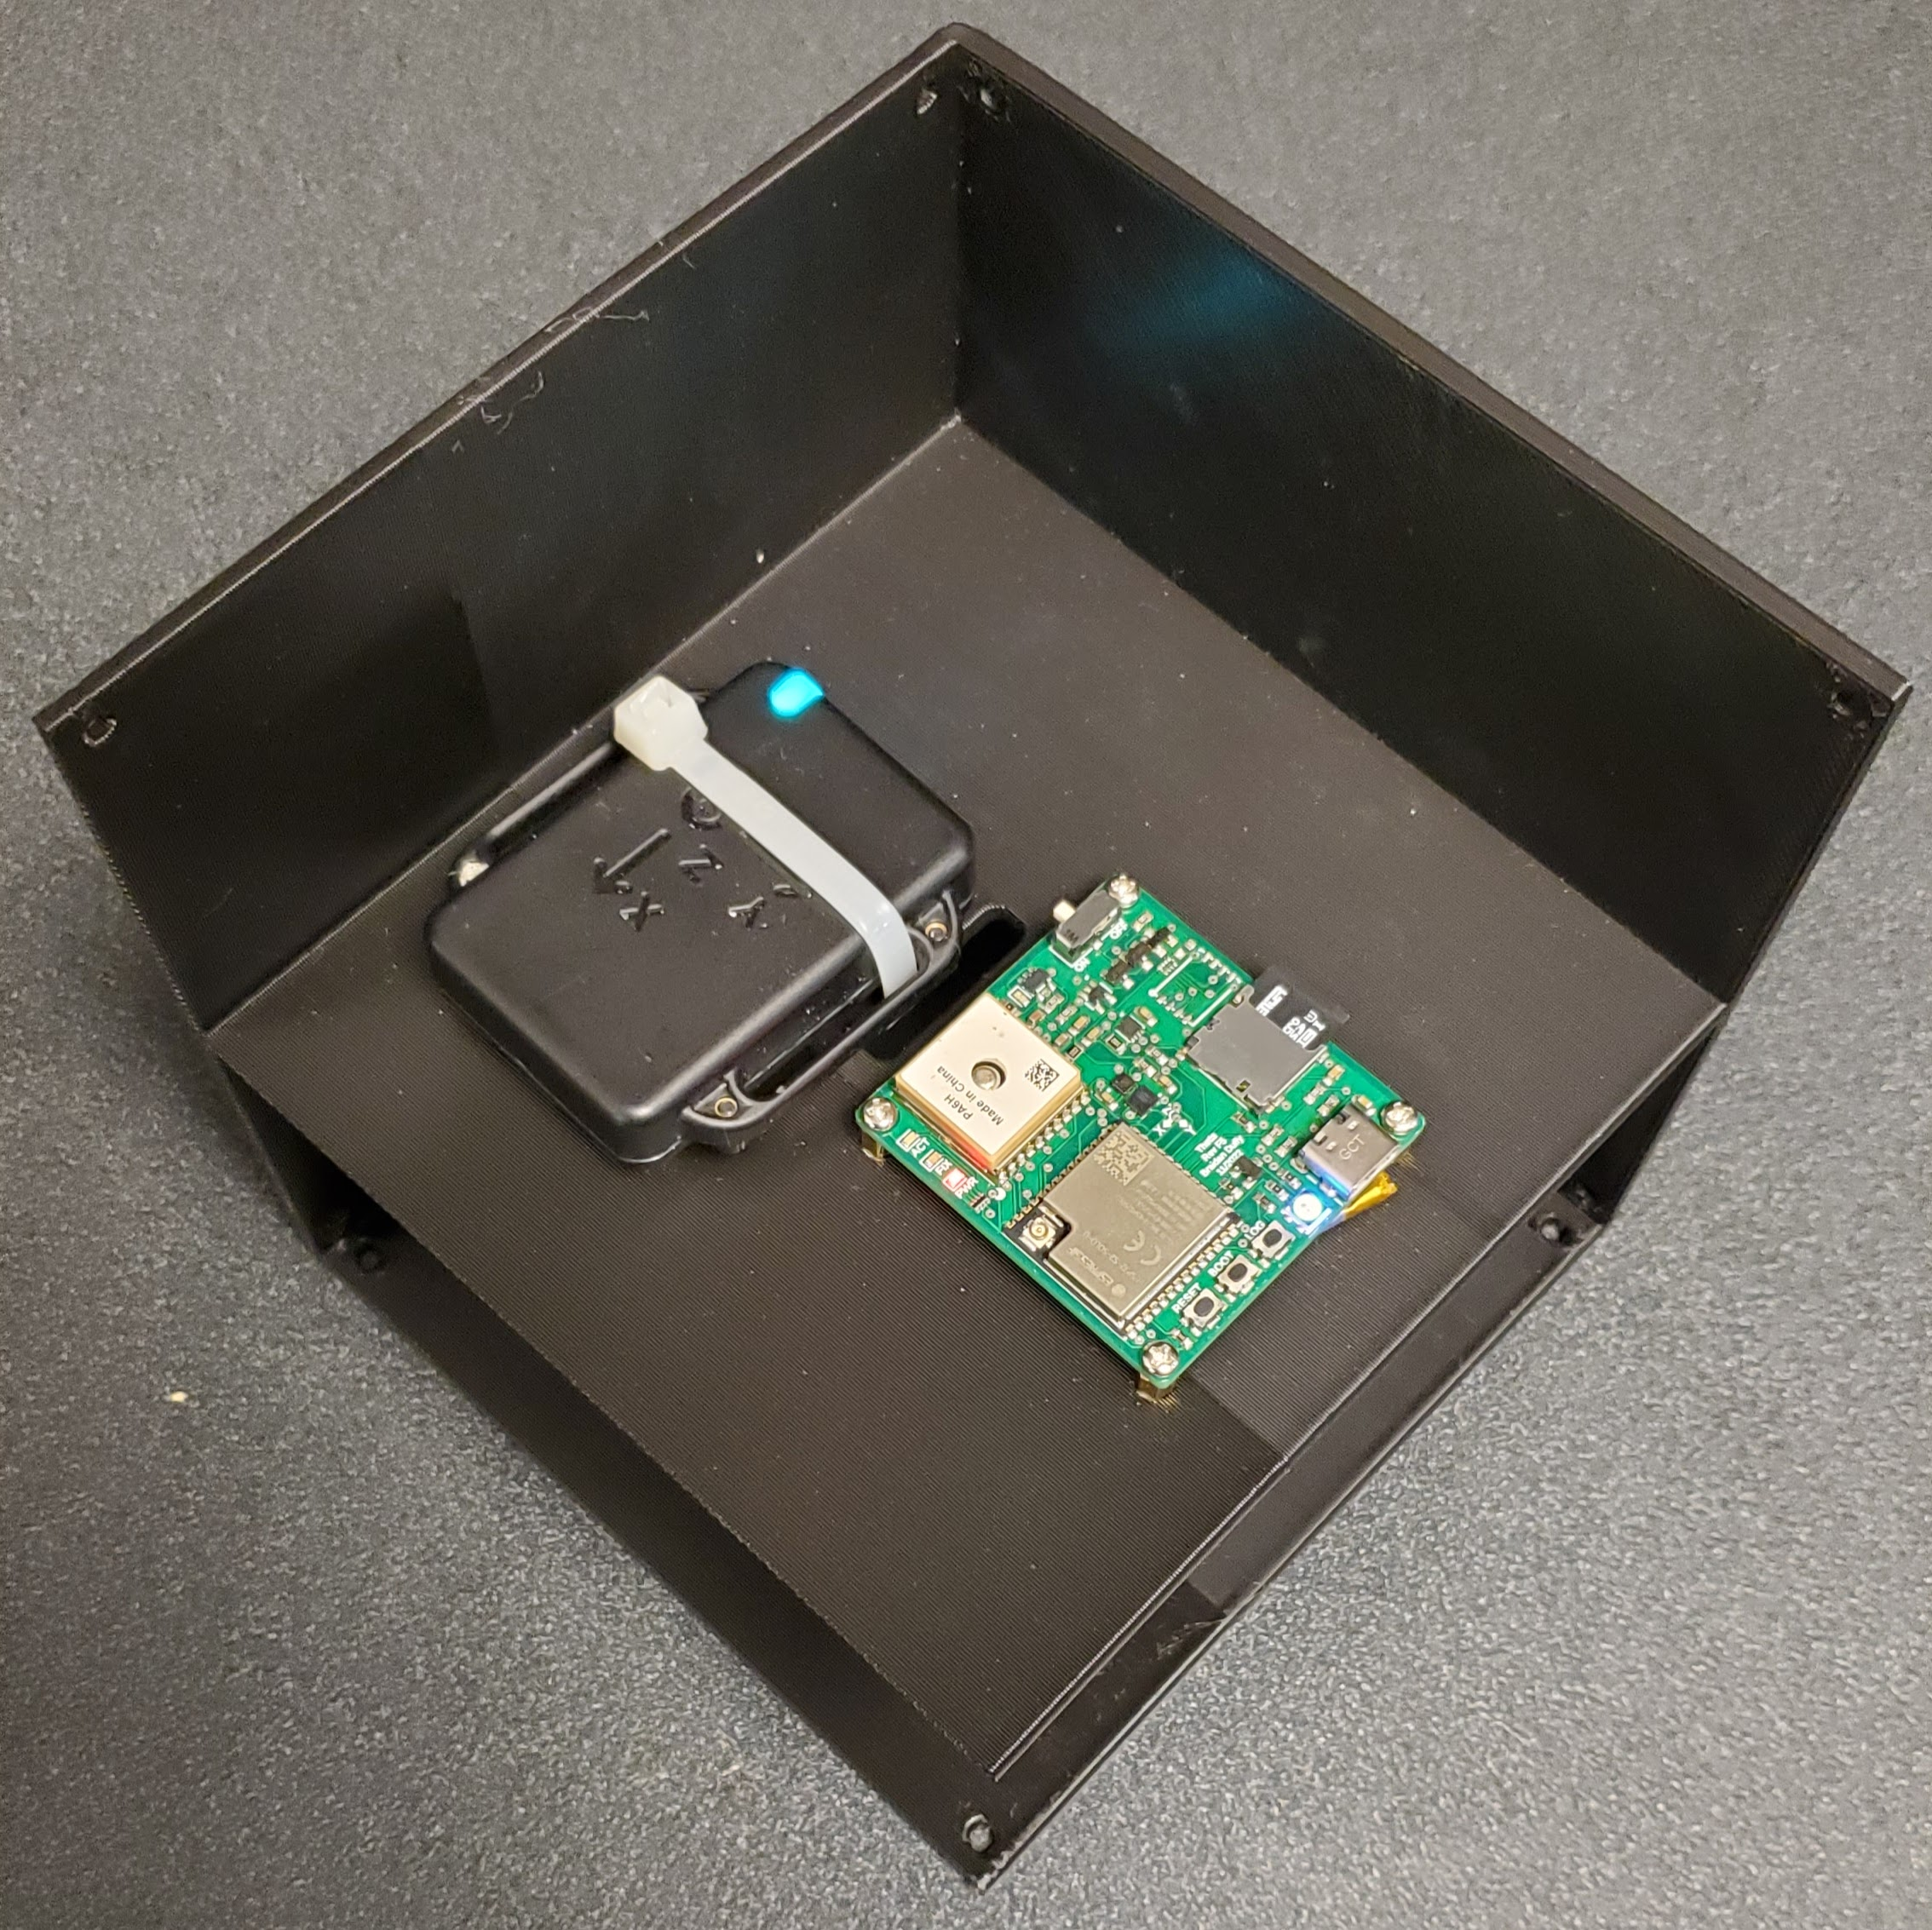
\includegraphics[height=2in]{calibration/calibration_cube2.jpg}
    \caption[Calibration cube]{Calibration cube with the x-IMU3 (left) and Thetis (right) mounted on it}
    \labfig{calibration_cube}
\end{figure}

To test the accelerometer and orientation data, a 72-tooth gear and socket was cut out of spare wood using a laser cutter.
With 72 teeth, the gear has a rotational resolution of 5-degrees per tooth with a high precision as the laser cut did not leave any room for play between the gear and socket.
This means that Thetis and the x-IMU3 can be rotated in 5-degree increments with a reasonably high presumption of accuracy.

\begin{figure}[h!]
    \centering
    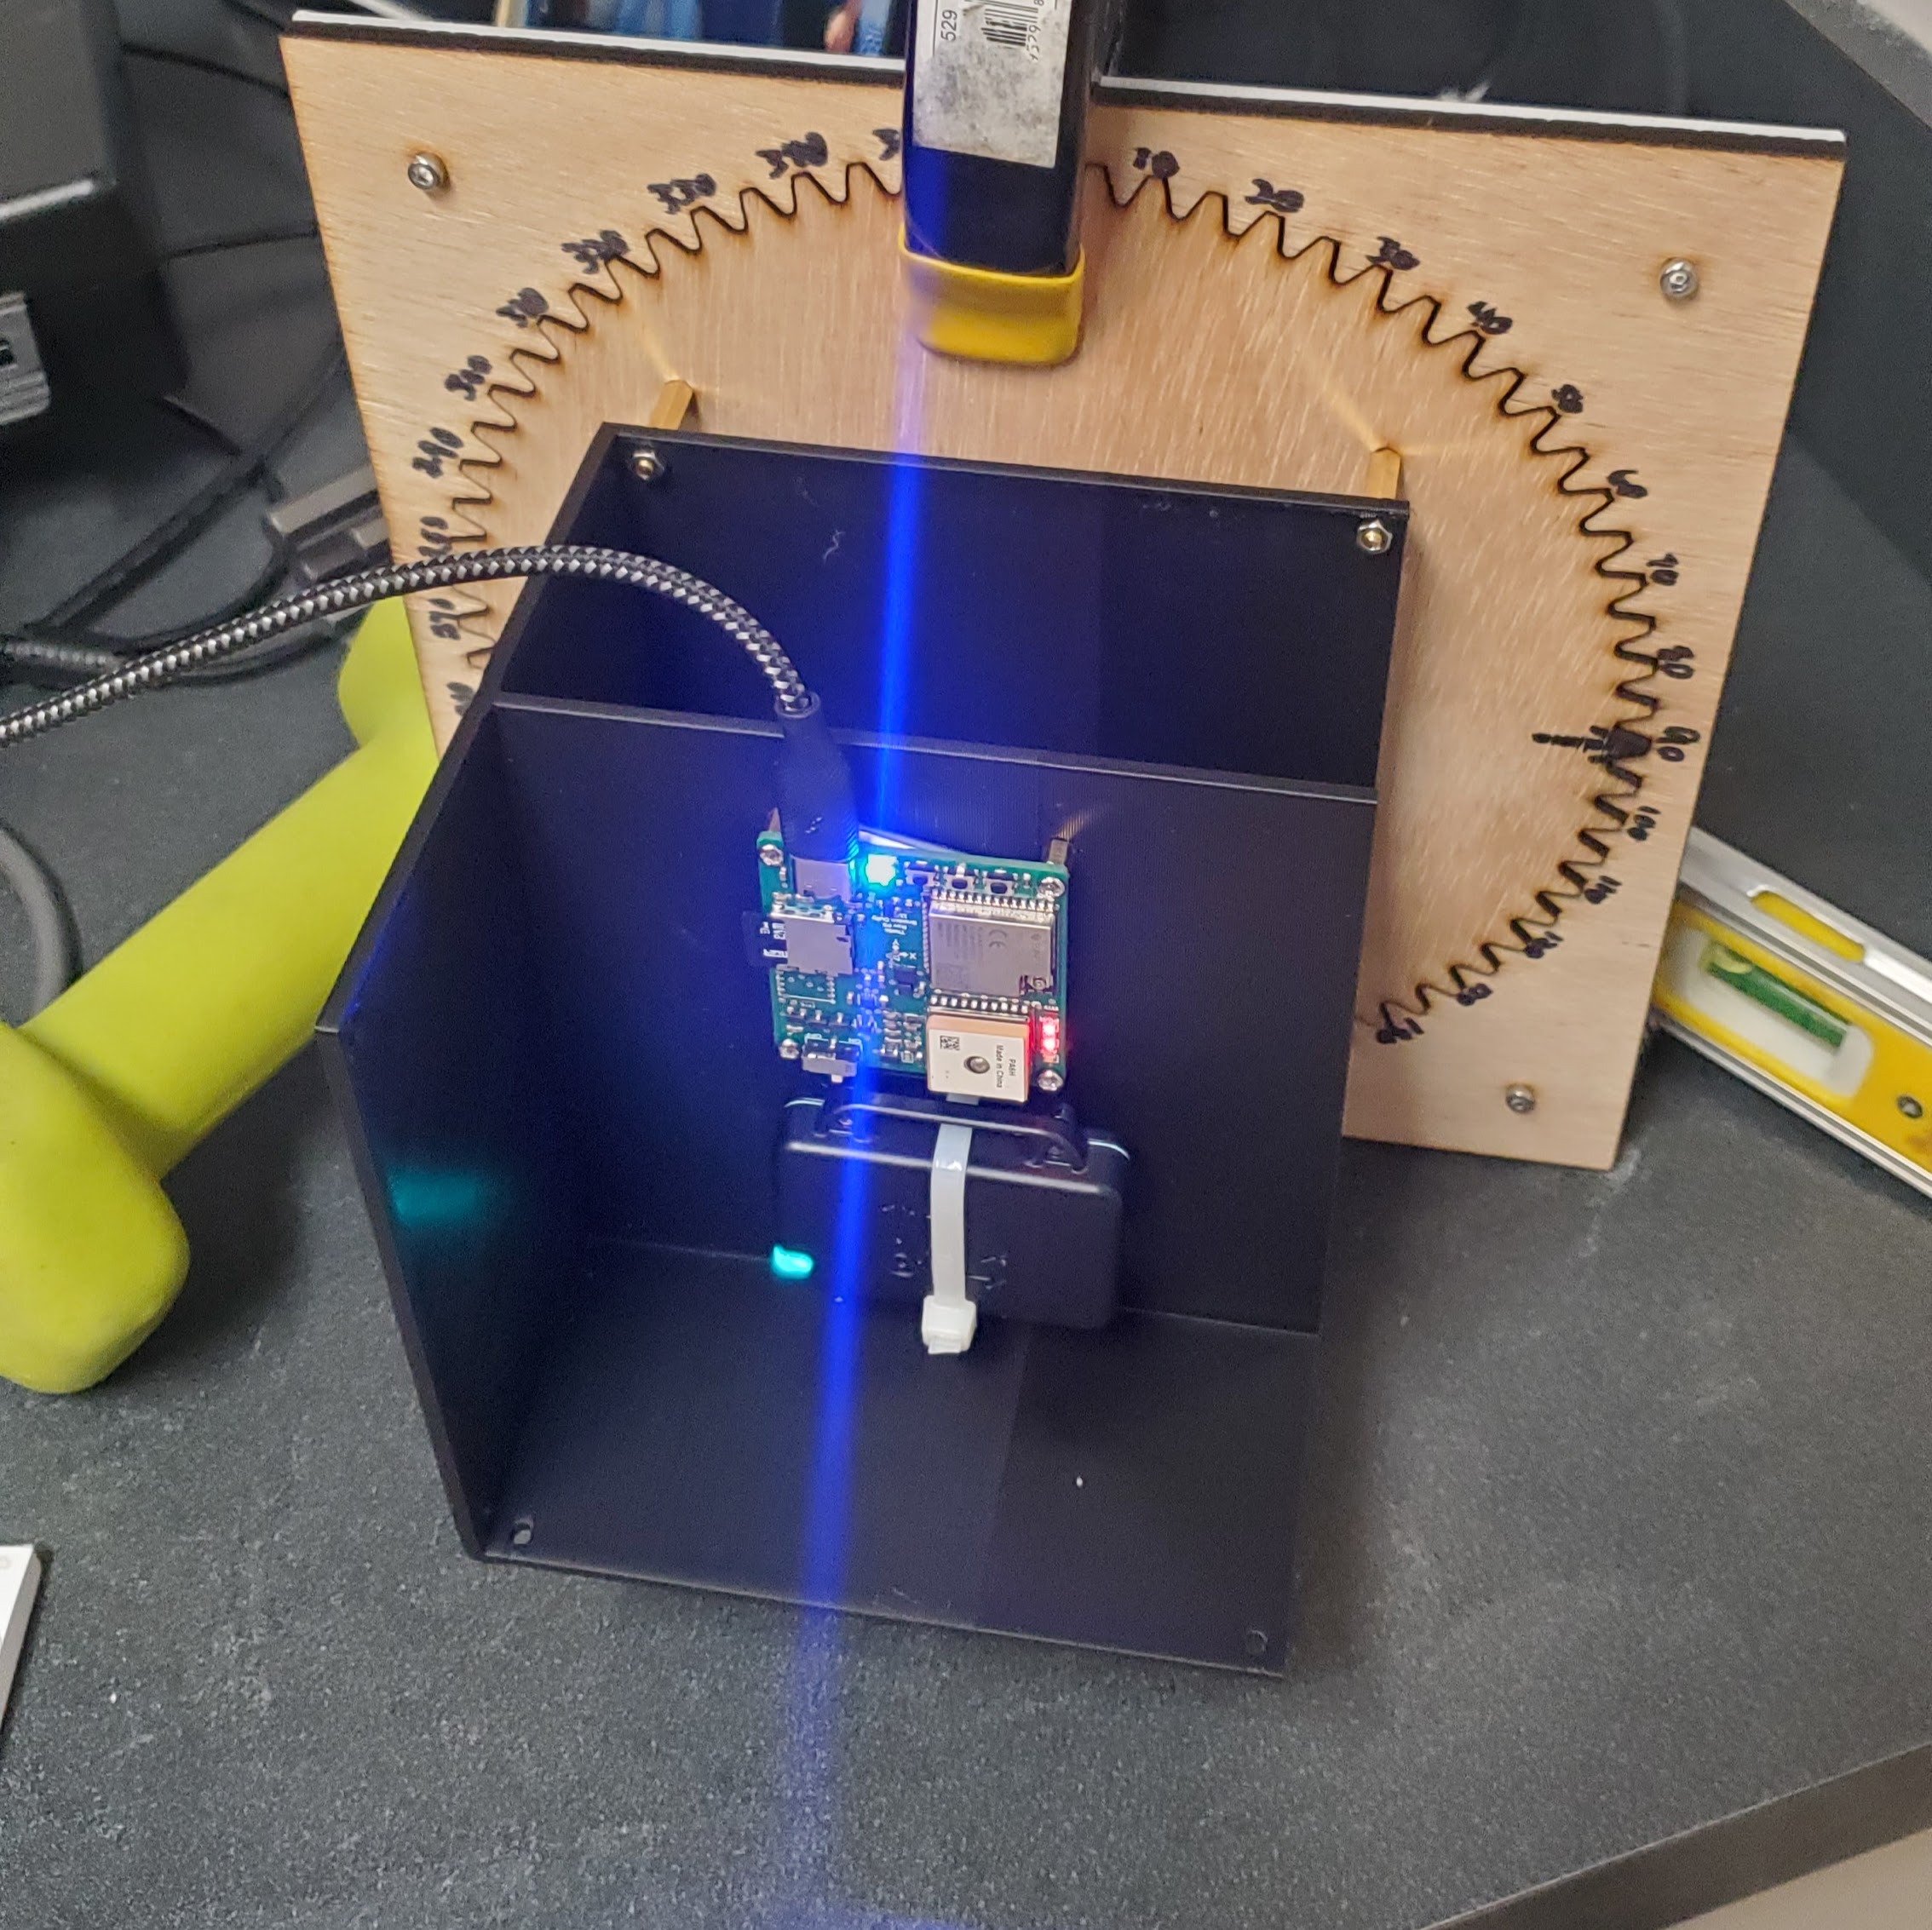
\includegraphics[height=2in]{calibration/calibration_cube_gear.jpg}
    \caption[Raw and Windowed Gyroscope Data]{Calibration cube mounted in the gear and socket apparatus for accelerometer and orientation testing.}
    \labfig{calibration_cube_gear}
\end{figure}

Finally, to test the gyroscope, a machine was designed and created that could rotate the calibration cube at a constant specified rate.
It is based on a Raspberry Pi running Robot Operating System 2 \cite{Macenski:2022} using a stepper motor driver HAT \footnote{\url{https://www.waveshare.com/stepper-motor-hat.htm}}.
The HAT is connected to a stepper motor which is coupled to a plate mounted on a lazy susan bearing \footnote{\url{https://www.tindie.com/products/fluxgarage/turntable-for-stepper-motor-kit/}}.
Commands to the Pi allow it to start the motor, begin rotating, and then stop rotating.
Some other features are implemented, but not used for calibration.

\begin{figure}[h!]
    \centering
    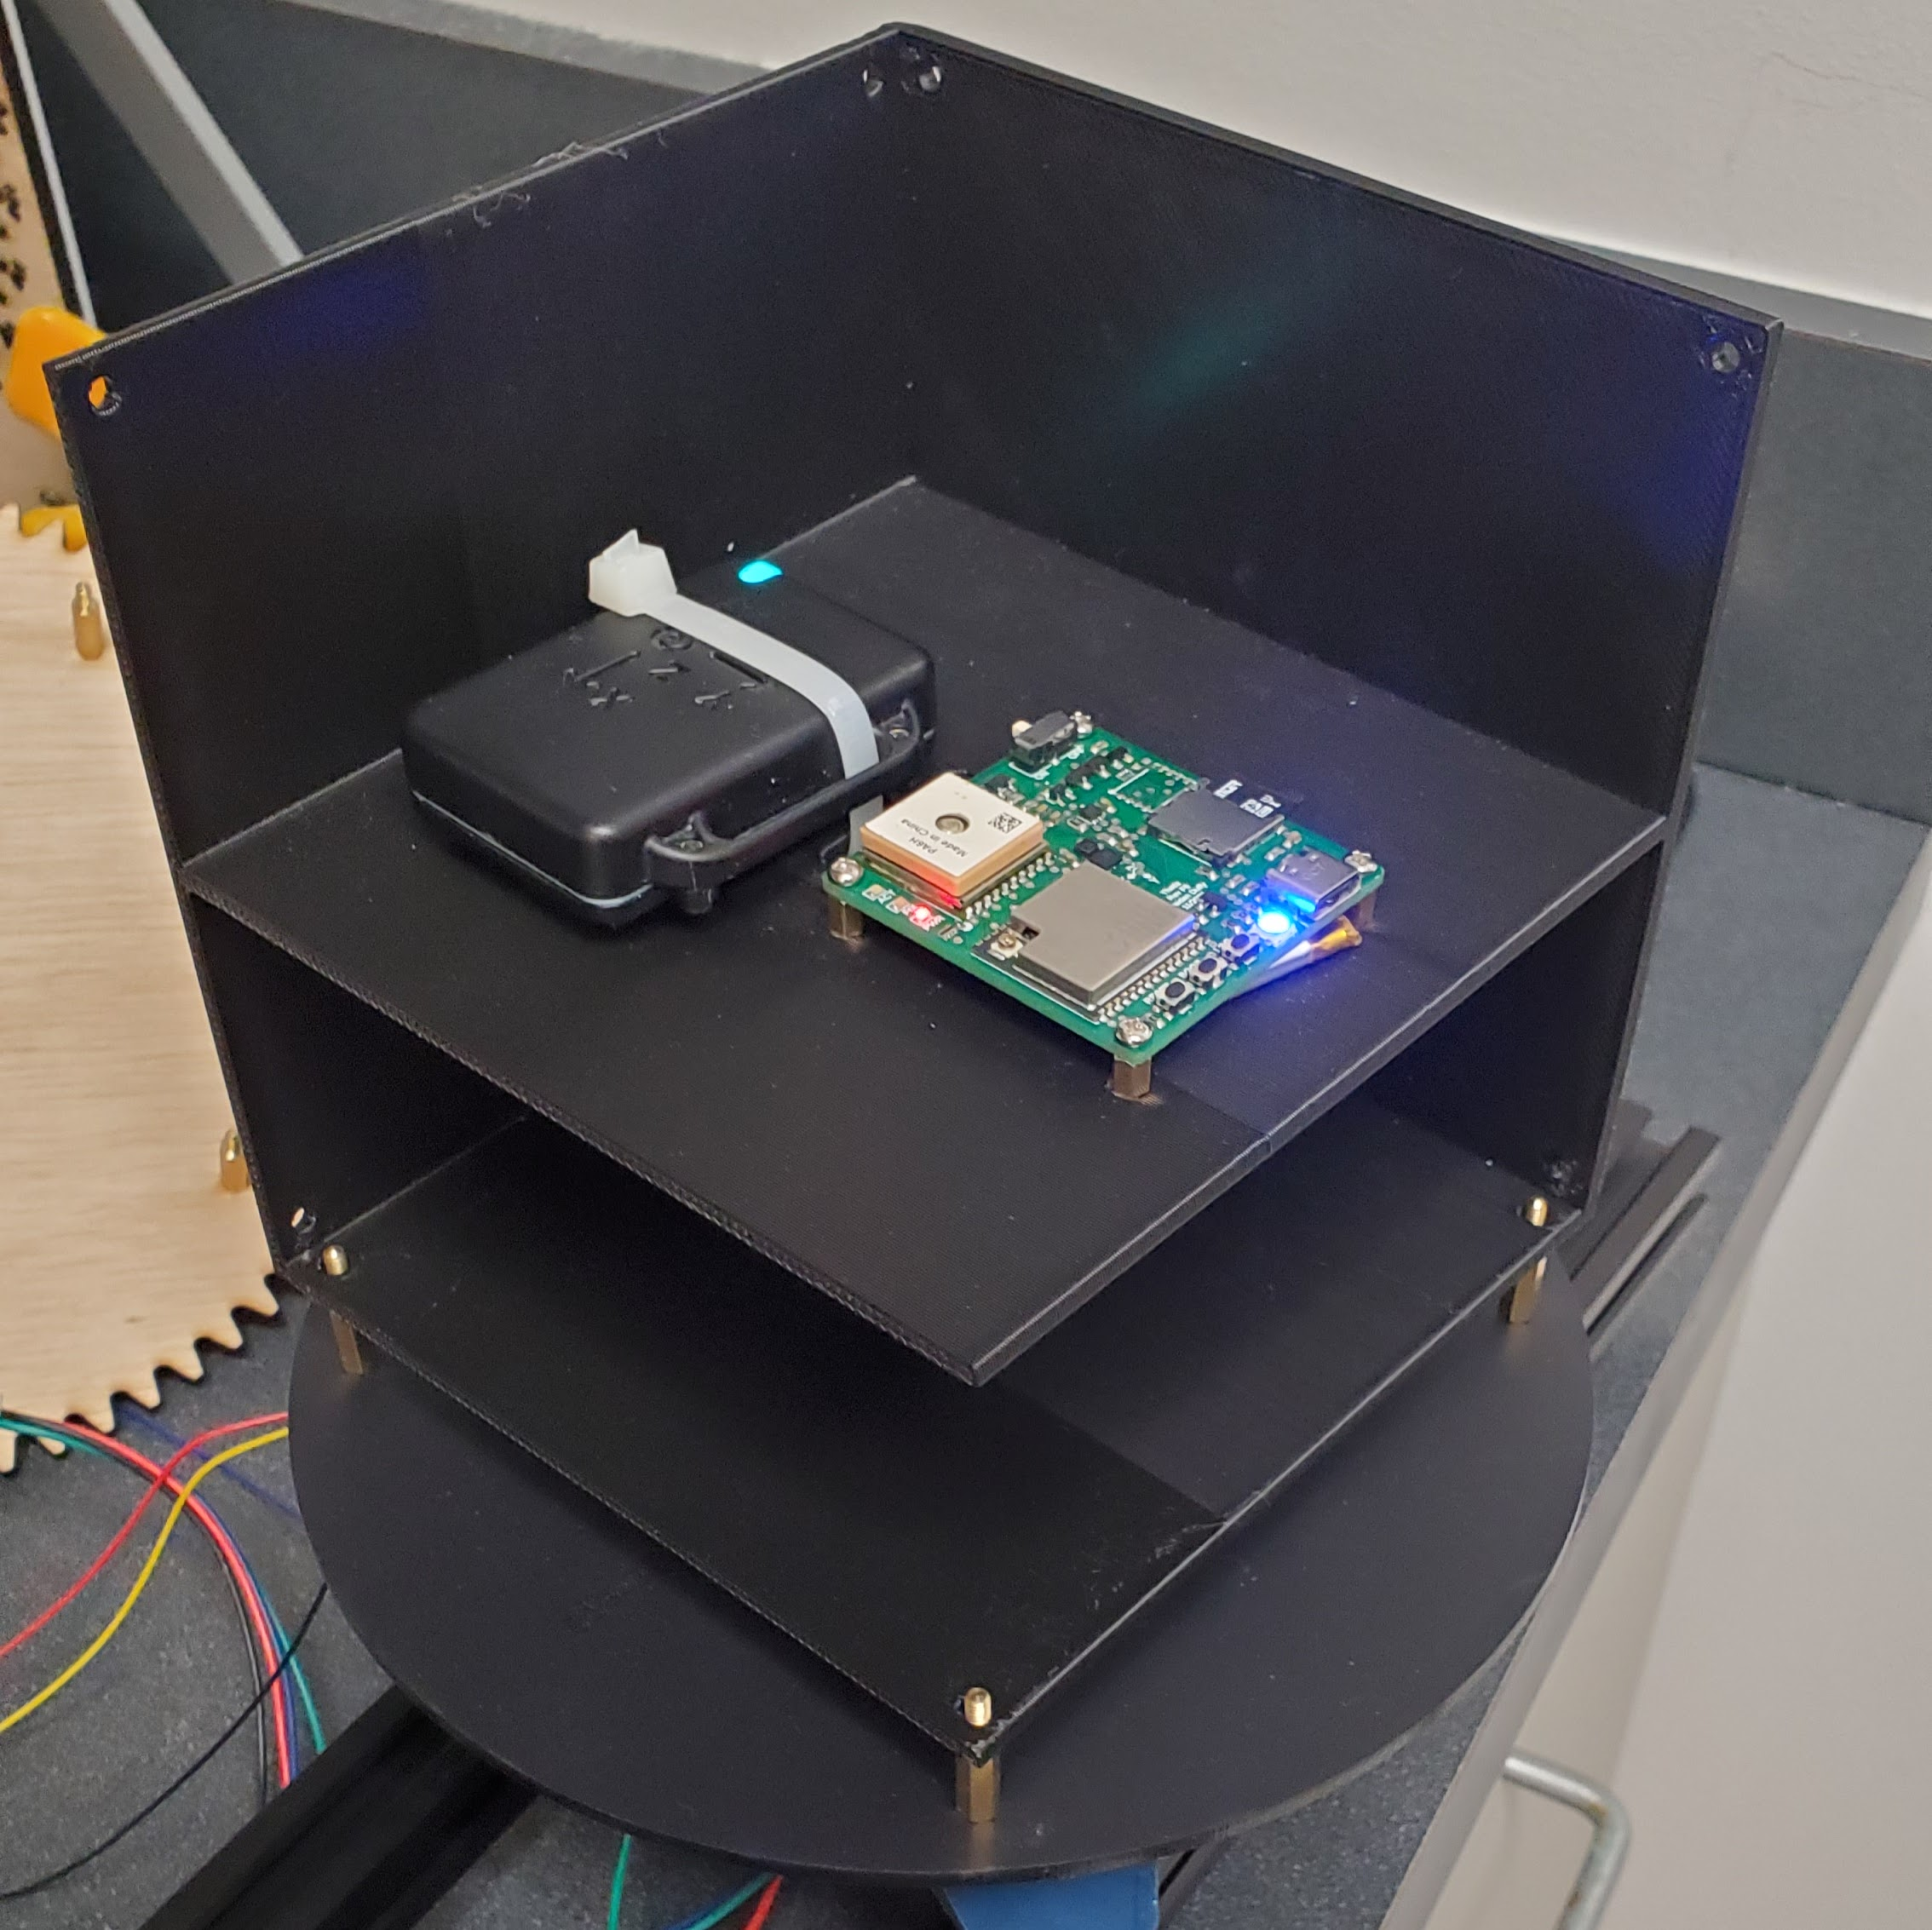
\includegraphics[height=2in]{calibration/calibration_cube_machine.jpg}
    \caption{Calibration cube mounted on top of the rotating plate for gyroscope data collection.}
    \labfig{calibration_cube_machine}
\end{figure}

\section{Methodologies} \labsec{calibration_methodologies}
The calibration process is important to improve the accuracy of the sensor before post processing and analysis are performed.
It is crucial that the calibration parameter settings on the device are at their default values before beginning.
Each of the starting misalignment ($M_0$) and soft iron ($W^{-1}$) matrices should be 3x3 identity matrices and the starting bias ($\pmb{b}$) and hard iron vectors ($\pmb{v}$) should be zero vectors.
Any starting sensitivity ($\pmb{s}$) vectors should also be a ones vector. 

\begin{gather}
    \pmb{b}_0 = [0, 0, 0] \\
    \pmb{s}_0 = [1, 1, 1] \\
    M_0 = 
    \begin{bmatrix}
    1 & 0 & 0 \\
    0 & 1 & 0 \\
    0 & 0 & 1 \\    
    \end{bmatrix} \\
    \pmb{v}_0 = [0, 0, 0] \\
    W^{-1} = 
    \begin{bmatrix}
        1 & 0 & 0 \\
        0 & 1 & 0 \\
        0 & 0 & 1 \\    
    \end{bmatrix}
\end{gather}

\subsection{Magnetometer} \labsubsec{calibration_magnetometer}
To calibrate the magnetometer, it needs to be rotated about all three axes in a "figure-8" motion.
This can be best accomplished by rotating about a single point while making the figure-8 pattern.
This ensures that the measurements in the X-, Y-, and Z-axis are evenly distributed throughout the magnetic field.
Without any distortions, this will create a sphere with a radius of the magnitude of the magnetic field.
However, as discussed in Chapter \ref{chap:background} and evidenced in Section \ref{sec:calibration_results}, this is not always the case.
To improve accuracy, make sure that the entire apparatus is far away from any magnetic influences such as electrical fields and magnets.

\subsection{Gyroscope} \labsubsec{calibration_gyroscope}
The gyroscope is calibrated using the calibration machine discussed more in Appendix \ref{chap:calibration_machine}. 
To begin, the machine must be booted and the measurement devices turned on.
Then, two terminal windows can be opened on the machine's Raspberry Pi through SSH or a headed setup.
On one terminal, navigate to the \lstinline[style=customInline]|calibrator_ws/| directory and execute the following command:

\begin{bash}
    source install/setup.bash && ros2 launch calibrator_bringup plate.launch.py
\end{bash}

\noindent This will start the ROS2 environment and allow the user to run the motor using the command line interface (CLI).
Ensure that the calibration machine is flat and level with the rotating plate horizontal as shown in Figure \ref{fig:calibration_cube_machine}.
When ready, set up the test by specifying the motor direction and speed in the second terminal window.
The former can be set using the command:

\begin{bash}
    ros2 service call /set_motor_dir calibrator_interfaces/SetBool "{data: <DIR>}"
\end{bash}

\noindent Where \lstinline[style=customInline]|DIR| is the desired direction - \lstinline[style=customInline]|true| will set the motor direction to clockwise, \lstinline[style=customInline]|false| will set the motor direction to counter-clockwise.
The motor speed can be set with the command:

\begin{bash}
    ros2 service call /set_motor_speed calibrator_interfaces/SetFloat64 "{data: <SPEED>}"
\end{bash}

\noindent Where \lstinline[style=customInline]|SPEED| is the desired test speed in degrees per second.
Note that it is not accurate and needs to be checked using an external tachometer.
For reference, calibration was done using three settings: 200, 300, and 400 which corresponded with the tachometer measurements of 305 deg/sec, 410 deg/sec, and 500 deg/sec, respectively.
To start the motor spinning, execute the command:

\begin{bash}
    ros2 service call /start_motor std_srvs/Trigger
\end{bash}

\noindent After a moment, the plate will begin spinning at your specified speed and direction.
Once you have collected the data, you can stop the motor using the command:

\begin{bash}
    ros2 service call /stop_motor std_srvs/Trigger
\end{bash}

\noindent After a few moments, the motor will come to a stop and the data can be offloaded.
Note that this command sets the motor speed to a default value, so you will need to reset the speed using the commands again.
It will be beneficial to start/stop recording at the start and end of every test so that a single log file represents a single test.

\subsection{Accelerometer} \labsubsec{calibration_accelerometer}
The accelerometer must be calibrated on the gear and socket apparatus while it is vertical.
The apparatus should be leveled such that the instruments on the calibration cube are perfectly vertical with respect to gravity and the other axes are planar to the Earth's surface.
Choose an axis and place the positive direction downwards (-1g).
The arrows on the coordinate reference markers point towards the positive direction.
Then, align the indicator on the gear with 0-degree marker on the socket, as shown in Figure \ref{fig:calibration_cube_gear}.

Rotate the calibration cube and gear in 45-degree increments, stopping for 30-seconds at each interval to collect an good average of data.
It will be beneficial to start/stop recording at the start and end of each increment so that a single log file represents a single orientation.

\subsection{Orientation} \labsubsec{calibration_orientation}
Roll and pitch orientation data can be collected simultaneously with the accelerometer calibration data as the devices are rotated about the X- and Y-axis, respectively.
This will give roll and pitch in 45-degree increments that can be analyzed for errors before and after calibration.

To get the yaw readings, we can re-use the gear and socket apparatus, this time placing it flat on a surface and placing the Z-axis of the devices vertical.
Make sure that the entire apparatus is far away from any magnetic influences and near the location where the magnetometer was calibrated.
Start the gear at the 0-degree marker on the socket, then orient the entire apparatus to magnetic north as determined by an external compass as shown in Figure \ref{fig:calibration_cube_compass}.
Rotate the calibration cube and gear in 45-degree increments for 360-degrees, pausing for 30-seconds at each interval to get an average reading.
It will be beneficial to start/stop recording at the start and end of each increment so that a single log file represents a single orientation.

\begin{figure}[h!]
    \centering
    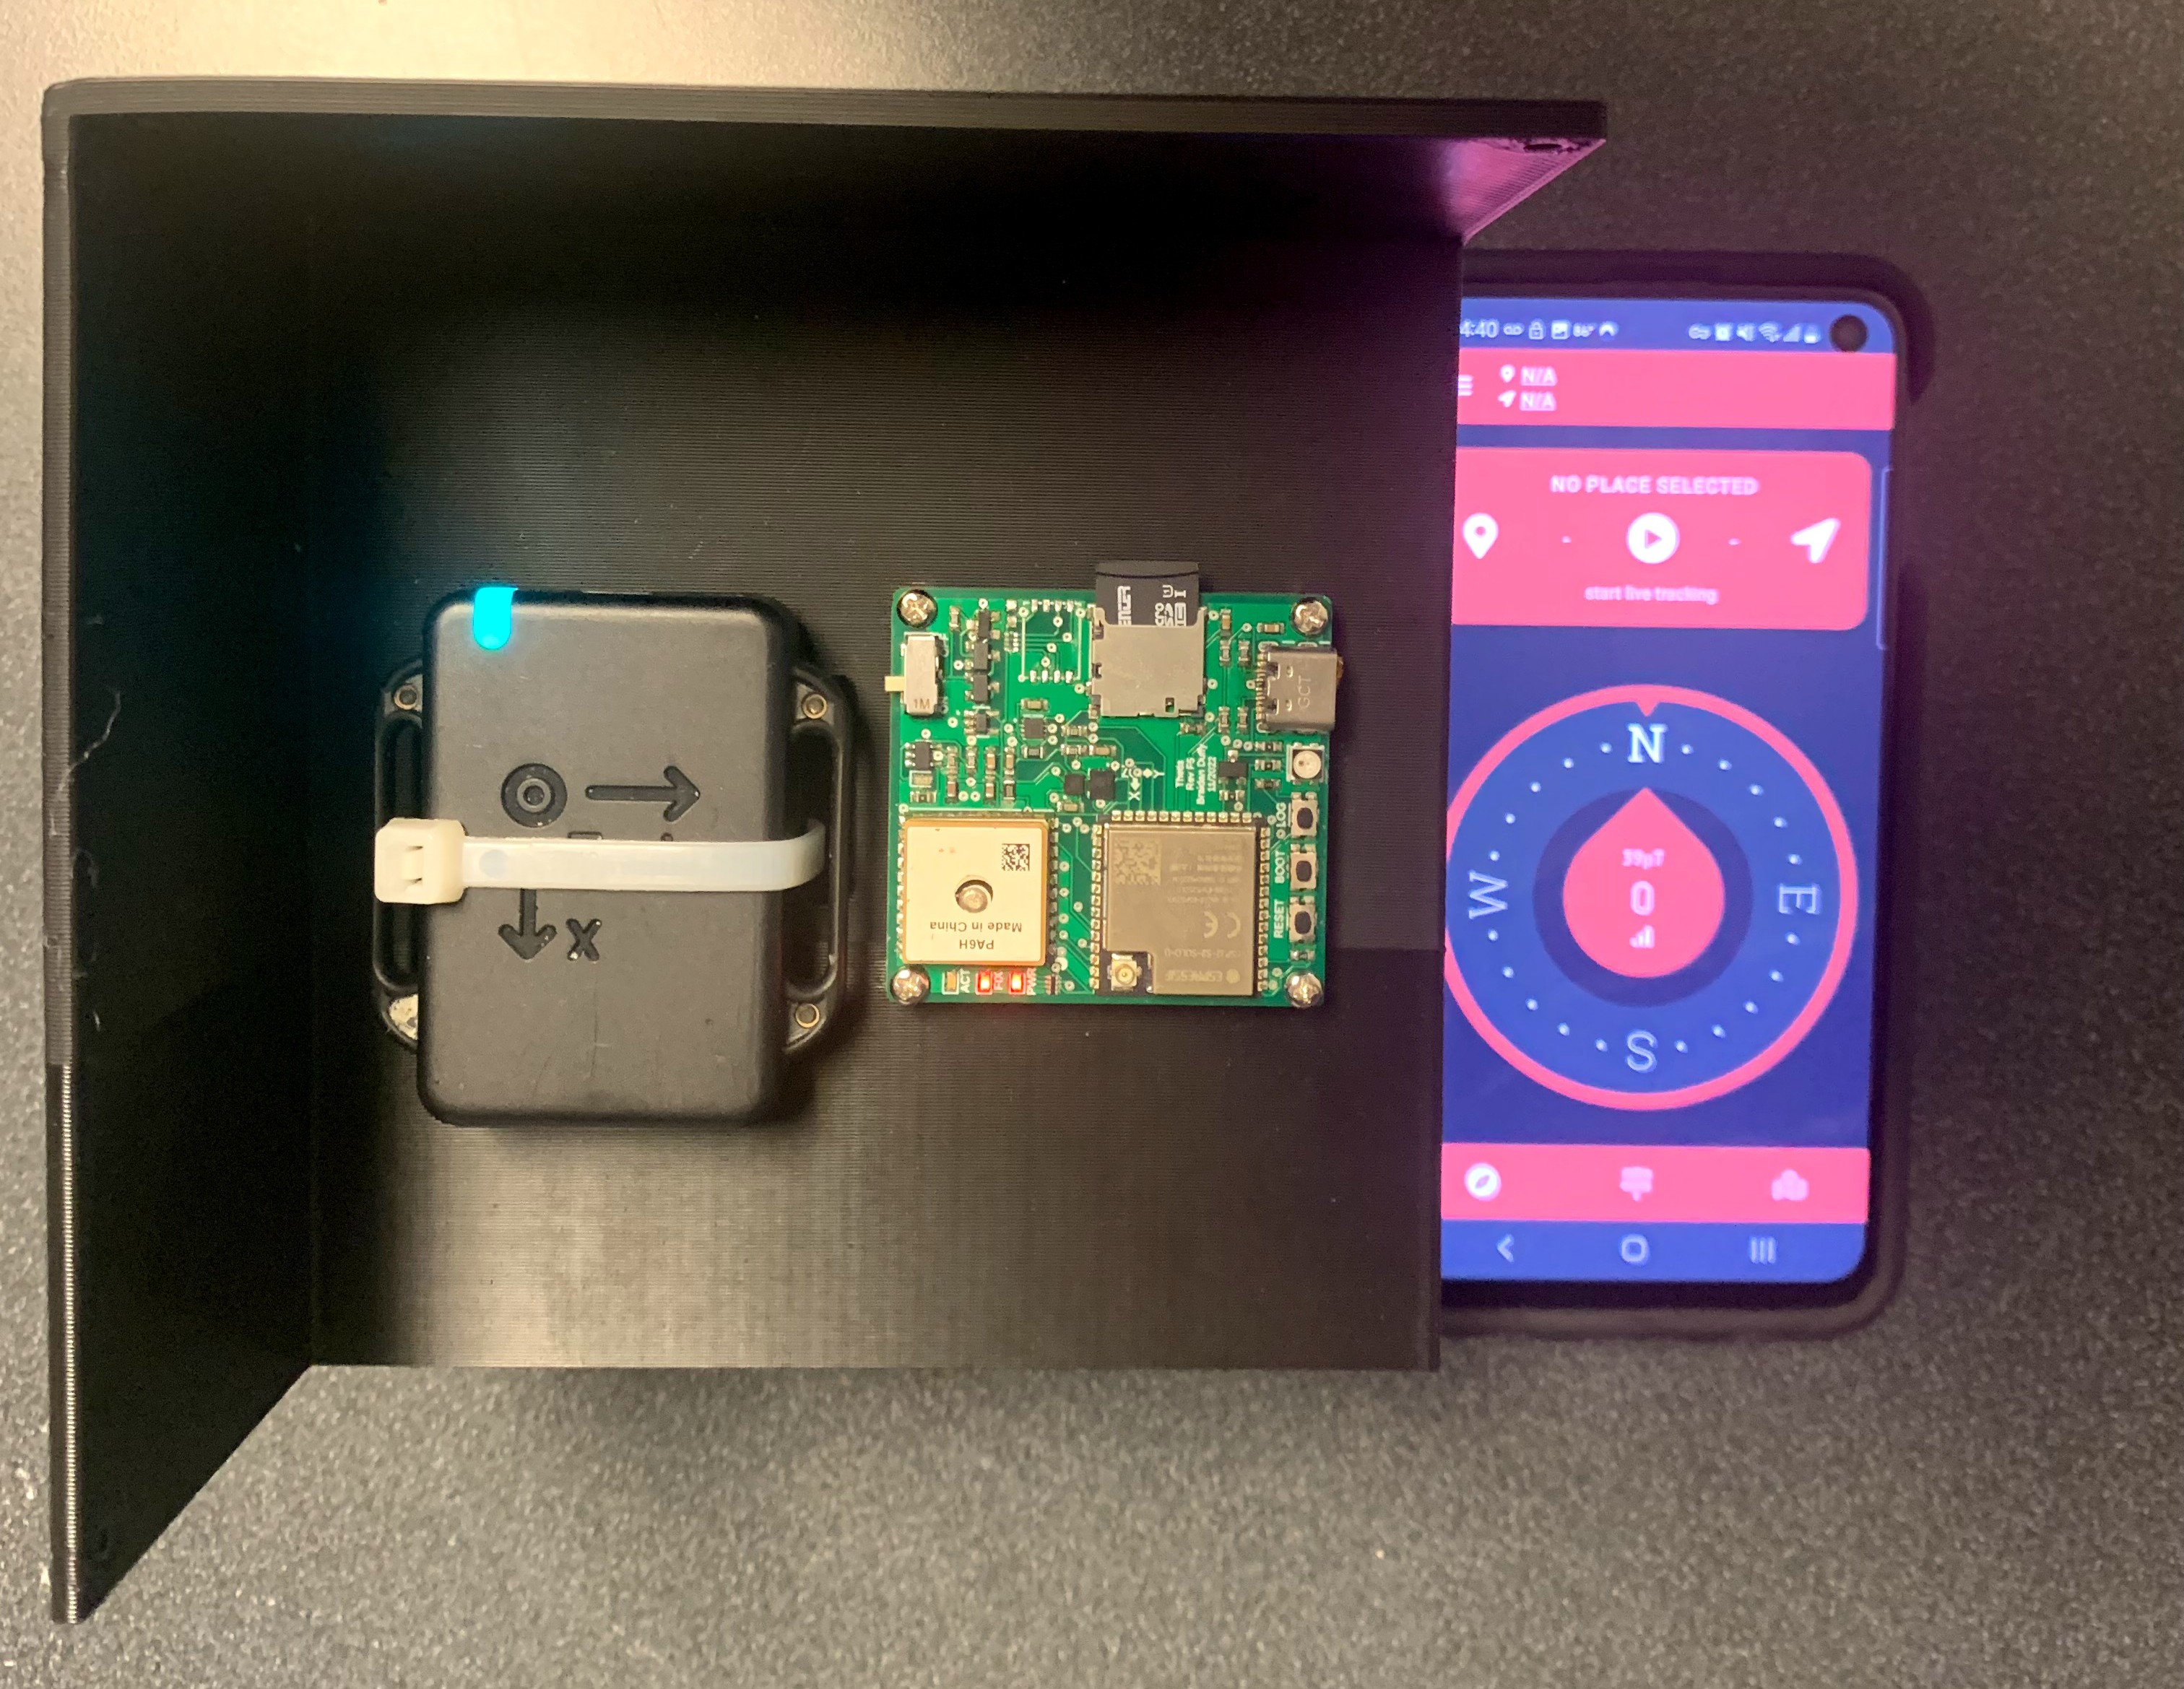
\includegraphics[height=2in]{calibration/calibration_cube_compass.jpg}
    \caption{Calibration cube aligned with an external compass.}
    \labfig{calibration_cube_compass}
\end{figure}

\section{Results} \labsec{calibration_results}
The calibration data was collected and ran through a calibration script in \cite{Thetis-Scripts}.
The raw log files were converted to CSVs using the x-IMU3 software conversion tool \footnote{\url{https://github.com/xioTechnologies/x-IMU3-Software/blob/main/Examples/Python/file_converter.py}}.
The resultant Magnetometer, Inertial, and Quaternion files were imported to the script using the \lstinline[style=customInline]|pandas| library.
Then, they were initially processed into dictionaries the contained the relevant data for each device for each test for each axis.

The raw data from each test dataset was cleaned by removing outliers and then windowed to an approximately 15-second span in the center of the data.
Windowing helped reduce processing time and automatically removed the heads and tails from the Thetis gyroscope plots, making analysis easier.
This cleaned and windowed data were placed back into the dictionary for each dataset and then plotted into the raw data figures shown in Appendix \ref{chap:raw_data_plots}.

After plotting the raw inertial data, the calibration parameters were calculated for the accelerometer and gyroscope.
The process used the mathematical techniques described in Chapter \ref{chap:background} and several external toolboxes.
For determining the misalignment matrix and sensitivity vector, the \lstinline[style=customInline]|scipy.optimize.minimize| toolbox was used with the Sequential Least Squares Programming (SLSQP) method.
For this method, the objective function defined in Equation \ref{eq:misalignment_obj_func} was used as the scalar function.

After producing the inertial calibration parameters, the script calculates the root-mean-square-error between for the devices with respect to ground truth and each other. 
These plots are shown in the following section.
After determining the inertial RMSE, the magnetic parameters are calculated using the previously discussed mathematical methods and several plots generated.

\subsection{Magnetometer}
This section shows the magnetometer calibration data as it is processed by the calibration script.
Note that the x-IMU3 does not have a hard or soft iron plot as it was already calibrated to remove these distortions.

\begin{figure}
    \centering
    \begin{subfigure}[b]{0.6\textwidth}
        \centering
        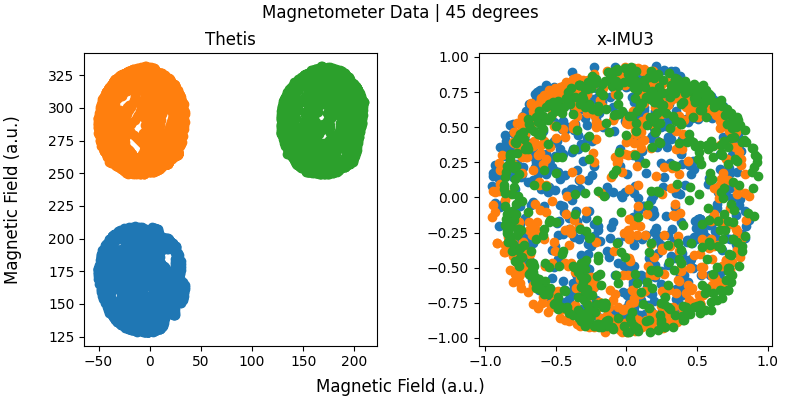
\includegraphics[width=\textwidth]{calibration/raw/raw_mag_all_45.png}
        \caption[Raw Magnetometer Readings]{Raw magnetometer calibration data from Thetis (left) and the x-IMU3 (right)}
        \labfig{mag_cal_raw}
    \end{subfigure}
    \hfill
    \begin{subfigure}[b]{0.3\textwidth}
        \centering
        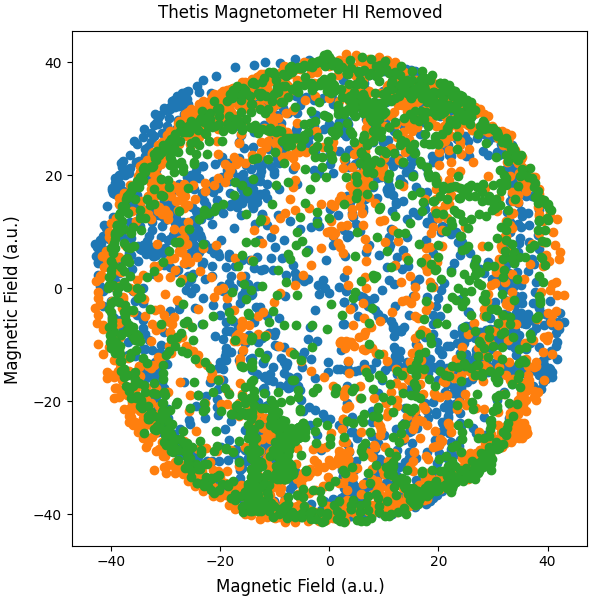
\includegraphics[width=\textwidth]{calibration/prelim/mag_hard_iron_removed.png}
        \caption[Hard Iron Distortion Removed]{Thetis magnetometer calibration data with hard iron distortion removed.}
        \labfig{mag_cal_hid_removed}
    \end{subfigure}
    \hfill
    \begin{subfigure}[b]{0.5\textwidth}
        \centering
        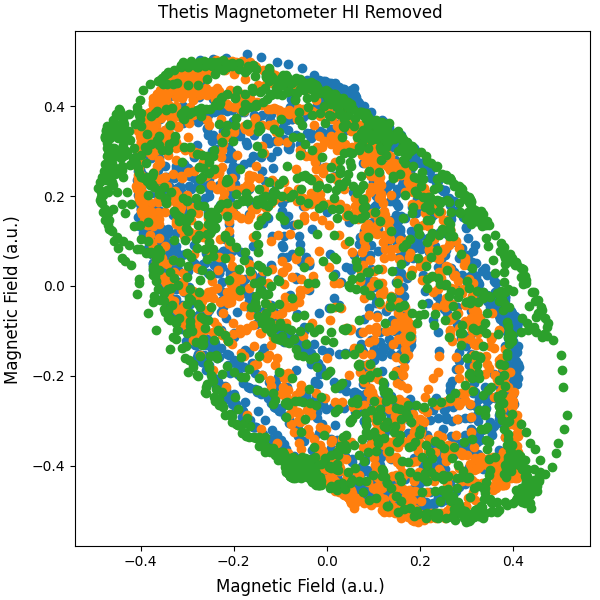
\includegraphics[width=\textwidth]{calibration/prelim/mag_soft_iron_removed.png}
        \caption[Soft Iron Distortion Removed]{Magnetometer calibration data with soft and hard iron distortion removed.}
        \labfig{mag_cal_sid_removed}
    \end{subfigure}
       \caption{Magnetometer calibration process}
       \labfig{magnetometer_calibration_process}
\end{figure}

The calibration data yielded the following parameters:

\begin{gather}
    \pmb{v} = \begin{bmatrix}
        -8.0752 \\
        168.7446 \\
        290.5438 \\
    \end{bmatrix} \\
    W^{-1} = \begin{bmatrix}
        0.0072 & -0.0040 & -0.0049 \\
        -0.0040 & 0.0100 & -0.0048 \\
        -0.0049 & -0.0048 & 0.0106 \\
    \end{bmatrix}
\end{gather}

\subsection{Gyroscope}

\begin{figure}
    \centering
    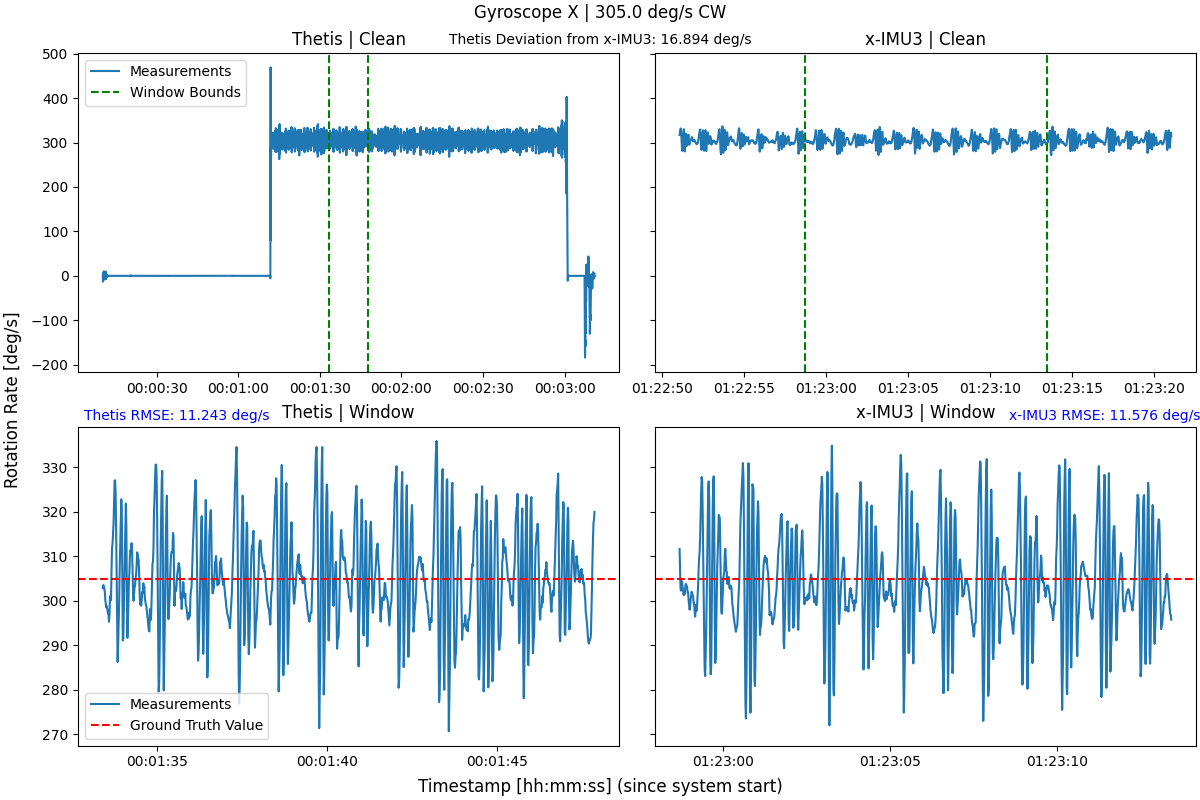
\includegraphics[width=\textwidth]{calibration/raw/raw_gyro_x-axis_305.png}
    \caption[Raw and Windowed Gyroscope Data]{Raw and windowed gyroscope data from Thetis (left) and the x-IMU3 (right).}
    \labfig{raw_gyro_data}
\end{figure}

\begin{figure}
    \centering
    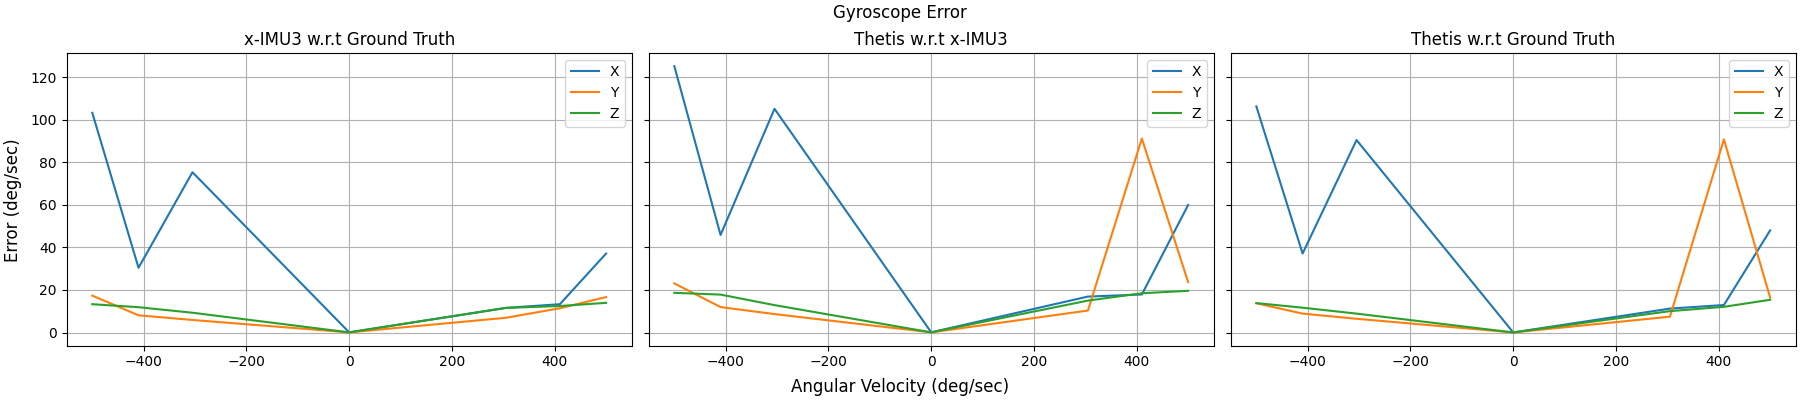
\includegraphics[width=\textwidth]{calibration/prelim/prelim_gyro.png}
    \caption[Cummulative Gyroscope Error]{Root-Mean-Square-Error during calibration across all axes and test speeds. From left to right, Thetis with respect to the ground truth, Thetis with respect to the x-IMU3, and the x-IMU3 with respect to the ground truth.}
    \labfig{prelim_gyro_data}
\end{figure}

The calibration data yielded the following parameters:

\begin{gather}
    \pmb{b} = \begin{bmatrix} \labeq{accelerometer_bias}
        -0.0003 \\
        0.0002 \\
        0.0002 \\
    \end{bmatrix} \\
    \pmb{s} = \begin{bmatrix} \labeq{accelerometer_sensitivity}
        1.0110 \\
        0.9672 \\
        1.0041 \\
    \end{bmatrix} \\
    M = \begin{bmatrix} \labeq{accelerometer_misalignment}
        1 & 0.0037 & 0.0399 \\
        0.0100 & 1 & -0.0075 \\
        -0.0259 & 0.0105 & 1 \\
    \end{bmatrix}
\end{gather}

\subsection{Accelerometer}

\begin{figure}
    \centering
    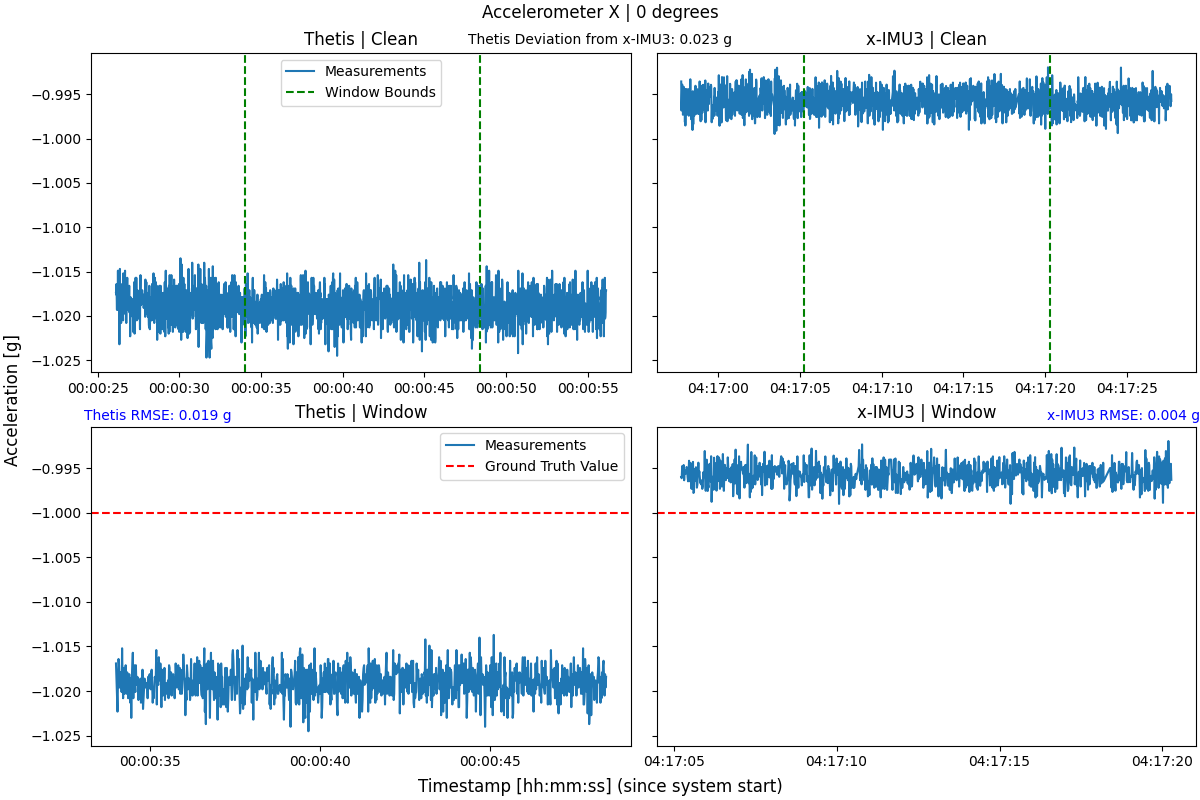
\includegraphics[width=\textwidth]{calibration/raw/raw_accel_x-axis_0.png}
    \caption[Raw and Windowed Accelerometer Data]{Raw and windowed accelerometer data from Thetis (left) and the x-IMU3 (right).}
    \labfig{raw_accel_data}
\end{figure}

\begin{figure}
    \centering
    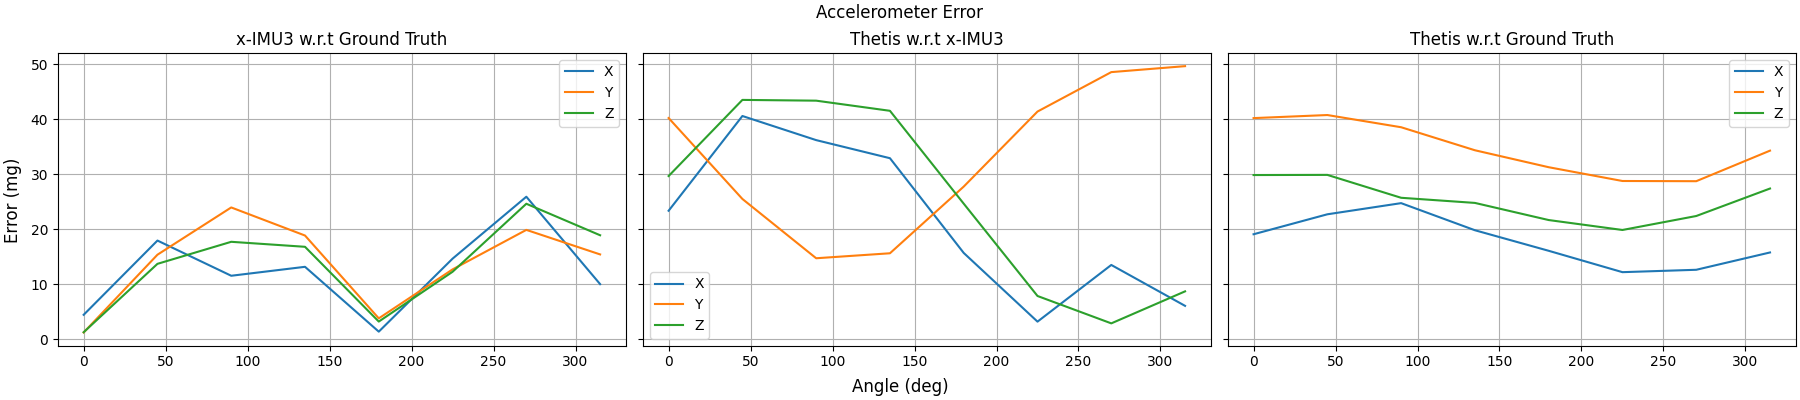
\includegraphics[width=\textwidth]{calibration/prelim/prelim_accel.png}
    \caption[Cumulative Gyroscope Error]{Root-Mean-Square-Error during calibration across all axes and test orientations. From left to right, Thetis with respect to the ground truth, Thetis with respect to the x-IMU3, and the x-IMU3 with respect to the ground truth.}
    \labfig{prelim_accel_data}
\end{figure}

The calibration data yielded the following parameters:

\begin{gather}
    \pmb{b} = \begin{bmatrix}
        -0.0243 \\
        0.0342 \\
        0.0112 \\
    \end{bmatrix} \\
    \pmb{s} = \begin{bmatrix}
        0.0171 \\
        0.6617 \\
        1.0022 \\
    \end{bmatrix} \\
    M = \begin{bmatrix}
        1 & 0.0033 & 0.0401 \\
        -0.3294 & 1 & -0.0067 \\
        -58.2018 & 0.0135 & 1 \\
    \end{bmatrix}
\end{gather}

\section{Discussion}
From the calibration results, we can identify several potential errors in the employed analytical methods.

\paragraph*{Magnetometer} First, regarding Figure \ref{fig:mag_cal_sid_removed}, the shape of the data points changes from spherical to ellipsoidal with a higher eccentricity than expected.
The measurements also decrease in intensity by two orders of magnitude. 
This indicates that 1) the Li ellipsoid fitting algorithm may not be applied using the correct radius for the target ellipsoid, and 2) that the target ellipsoid has too high of eccentricity to be fitted into a sphere.
Identifying and implementing a fix to this issue is currently out of the scope of this thesis due to time constraints.
Therefore, it is recommended that only the hard iron offset, $\pmb{v}$, be used for calibrating magnetic measurements for now.

With the hard iron offset applied to the data, the following RMSE values and per cent errors are reported:

\begin{table}[h!]
    \renewcommand{\arraystretch}{1.75}
    \centering
    \begin{tabular}{| m{5cm} | c | c |}
        \hline
        \textbf{Comparison} & \textbf{RMSE (uT)} & \textbf{Percent Error} \\
        \hline
        Thetis w.r.t Ground Truth\footnote{As measured curing calibration, the magnitude of the magnetic field was ~45 uT} & 3.49 & 7.33\% \\
        Thetis w.r.t x-IMU3\footnote{From the x-IMU3 data sheet, the x-IMU3 readings were converted from a.u. to uT using 50 uT/a.u.} & 4.92 & 9.34\% \\
        x-IMU3 w.r.t Ground Truth\footnotemark[\value{footnote}] & 2.48 & 4.69\% \\
        \hline
    \end{tabular}
\end{table}

We can see a larger deviation from Thetis with respect to the ground truth and the x-IMU3, but the couple of percentage points difference between Thetis and the x-IMU3 could be caused by sensor performance and the x-IMU3's application of soft iron distortion compensation.

\paragraph*{Gyroscope} In the gyroscope calibration data, we can see a lot of error introduced via noise into the measurements.
The calibration machine does not spin at a constant rate and seems to have an induced oscillation and variance as the plate rotates.
Additionally, the calibration cube's moment of inertia is not centered directly on the rotation axes because the object is not weighted symmetrically.
These errors lead to the large RMSE values shown in Figure \ref{fig:prelim_gyro_data} between Thetis and the x-IMU3.
The large noise magnitudes for some of the X- and Y-axis tests also introduced exceedingly large errors for the calibration data upwards of 100 deg/sec (~20\%).

The errors are consistent across the Thetis and x-IMU3 datasets suggesting that they are systematic errors with the calibration machine, and not any one sensor itself.
When the machine seems to work properly, with minimal noise in the data set, the error in Thetis and x-IMU3 with respect to each other and the ground truth varies between 5\% and 10\% which is within reason given that Thetis is uncalibrated and not accounting for any measurement errors itself.
If the machine was more stable and able to give more useful data, the calibration parameters could be calculated better and applied to reduce Thetis's measurement error.
However, because of the large discrepancies in the calibration data and error, it is not recommended to use the calculated calibration parameters for the gyroscope.

\paragraph*{Accelerometer} The accelerometer calibration data looks good at first glance except for the average error being several tenths of a g.
Even on the x-IMU3, the error remains higher than provided in the calibration certificate, implying that there are errors in the test apparatus.
Most likely, the gear and socket were not perfectly flat and aligned with the gravitational field.
Therefore, the other axes sensed the gravitational field more and caused the readings on the sensing axis to skew.
The error persisted throughout all angles of testing on all axes as shown in Figure \ref{fig:prelim_accel_data}, further reinforcing the theory that it was introduced by the testing apparatus rather than the instruments themselves.

A very concerning problem are the misalignment matrix and sensitivity vector calculated from the calibration data.
The sensitivity vector, $\pmb{s}$, should have values around 1.
The x-IMU3 calibration certificate shows that the sensitivity vectors for that device are within 1\% of normal.
The calculated values shown in Equation \ref{eq:accelerometer_sensitivity} are significantly less than 1, meaning that the measurements will not be near their true value.
Additionally, the misalignment matrix should have values that are near zero surrounding the diagonal 1's.
The value of $M_{31}$ is $-58.2018$ which strongly indicates this calibration was not successful.

The most likely reason these discrepancies have occurred is because of the method from which the sensitivity and misalignment matrices are calculated.
They are calculated using a non-linear optimization algorithm that tries to minimize the error found in an objective function (Equation \ref{eq:misalignment_obj_func}).
As the minimization occurs, it can fall into local minima that fulfill the boundary conditions laid out for this methodology, but will result in invalid calibration parameters.
Further research needs to be performed on the best optimization techniques to find these calibration parameters.
This research is out of the scope of the thesis due to the technical involvement and time constraints.
Based on these errors, it is not recommended to use the accelerometer calibration parameters calculated here.

\paragraph*{Conclusion} Due to errors in the inertial data collection and analytical methods, Thetis cannot have its accelerometer or gyroscope calibrated at this time.
However, the magnetometer can be calibrated using only the hard iron offset.
The calibration data taken between Thetis and the x-IMU3 suggests that the devices perform closely with one another and that given more time and expertise with calibration, Thetis can become reasonably equivalent to the x-IMU3 in terms of sensor performance under the methodologies described above.
The data collection process also demonstrated that Thetis can collect measurements reliably via its on board SD card storage and that can be offloaded and post-processed.
The data was collected at 64 Hz sample rate which also validated some system requirements - this will be further explained in the next chapter.